\documentclass[11pt]{article}
\bibliographystyle{unsrtnat}
\usepackage{tabularx} 
\usepackage{subfigure}
\usepackage{caption}
\usepackage{url}
\usepackage{graphicx}
\usepackage{multirow}
\usepackage{amsmath} 
\usepackage{physics}
\usepackage{bm}
\newcommand{\uvec}[1]{\boldsymbol{\hat{\textbf{#1}}}}
\usepackage{graphicx}
\usepackage[margin=1in,letterpaper]{geometry} 
\usepackage[final]{hyperref}
\hypersetup{
	colorlinks=true,
	linkcolor=blue,
	citecolor=black,
	filecolor=magenta,
	urlcolor=blue         
}
\begin{document}
\title{\textbf{\Huge Solar winds}}
\author{Erlend Syljuåsen}
\date{Norwegian University of Science and Technology\\spring 2022}
\maketitle

\begin{abstract}
\begin{center}
Solar wind was modelled by protons moving in earths magnetic field. Trajectories for three different velocities has been plotted and discussed.
\end{center}
\end{abstract}

\section{Theory}
A pure dipole centered at the origin produces a magnetic field
$$\vectorbold{B}(\vectorbold{r}) = \frac{\mu_0}{4\pi} \left(\frac{3\vectorbold{r}(\vectorbold{m} \cdot \vectorbold{r})}{r^5} - \frac{\vectorbold{m}}{r^3}\right)$$
The equation of motion, given by the Lorentz force where $\vectorbold{E} = 0$ is 
$$\ddot{\vectorbold{r}} = \frac{q}{m} \dot{\vectorbold{r}} \times \vectorbold{B}$$
Introducing dimensionless variables $\tilde{\vectorbold{r}}= \frac{\vectorbold{r}}{r_0}$, $\tilde{\vectorbold{m}} = \frac{\vectorbold{m}}{m_0}$, $\tilde{t}= \frac{t}{t_0}$, the equation of motion can be rewritten to
\begin{equation}
    \frac{d^2 \tilde{\vectorbold{r}}}{{d\tilde{t}}^2} = \frac{d\tilde{\vectorbold{r}}}{d\tilde{t}} \times \tilde{\vectorbold{B}}
    \label{eq:diff}
\end{equation}
where $$\tilde{\vectorbold{B}} = C\frac{3 \hat{\tilde{\vectorbold{r}}} (\tilde{\vectorbold{m}} \cdot \hat{\tilde{\vectorbold{r}}}) - \tilde{\vectorbold{m}}}{{\tilde{r}}^3}$$ 
and $$ C = \frac{q_{proton}\mu_0 m_0}{m_{proton} 4 \pi \tilde{v_0} {r_0}^2}$$
The constant C has been chosen such that $\frac{d\tilde{\vectorbold{r}}}{d\tilde{t}}|_{\tilde{t}=0}= \tilde{v_0}$. The constants used are displayed in the table below.
\begin{center}
\begin{tabular}{|c|c|c|c|c|c|c|}
\hline
    constant & value & dimension\\
\hline
    $r_0$ & $6371 \cdot 10^3$ & m\\ 
    $m_0$ & $8.22 \cdot 10^{22}$ & Am$^2$\\ 
    $q_{proton}$ & $1.6 \cdot 10^{-19}$ & C\\
    $m_{proton}$ & $1.67 \cdot 10^{-27}$ & kg\\
\hline
\end{tabular}
\label{table:constants}
\end{center}

\section{Implementation}
By rewriting \eqref{eq:diff} we obtain two first order differential equations
\begin{equation}
    \frac{d\tilde{\vectorbold{r}}}{d\tilde{t}} = \tilde{\vectorbold{v}}\\
    \hspace{10mm} \frac{d\tilde{\vectorbold{v}}}{d\tilde{t}} = \tilde{\vectorbold{v}} \times \tilde{\vectorbold{B}} 
\end{equation}
In the implementation $\vectorbold{\Lambda}$ is the solution matrix which contains both $\tilde{\vectorbold{v}}$ and $\tilde{\vectorbold{r}}$ for all timesteps. The ODE can then be written as $$\frac{d}{d\tilde{t}} [\tilde{\vectorbold{r}}, \tilde{\vectorbold{v}}]^T = \frac{d\vectorbold{\Lambda}}{d\tilde{t}} = f(\vectorbold{\Lambda}) = [\tilde{\vectorbold{v}}, \tilde{\vectorbold{v}} \times \tilde{\vectorbold{B}}]^{T}$$
Runge-Kutta-Fehlberg method has been chosen as a suitable ODE solver. The implementation can be found at github \cite{erlensy_github}.

\section{Results and discussion}
In figure \ref{fig:mag_field} the magnetic field of the earth has been visualized in two different planes.
\begin{figure}[!htp]
    \centering
    \captionsetup{justification=centering}
    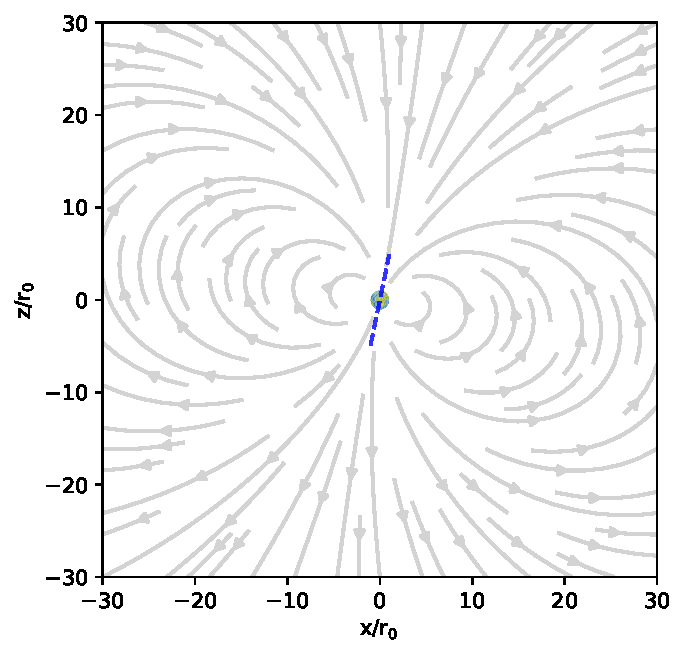
\includegraphics[width=0.49\textwidth]{../figures/report/magFieldXZ}
    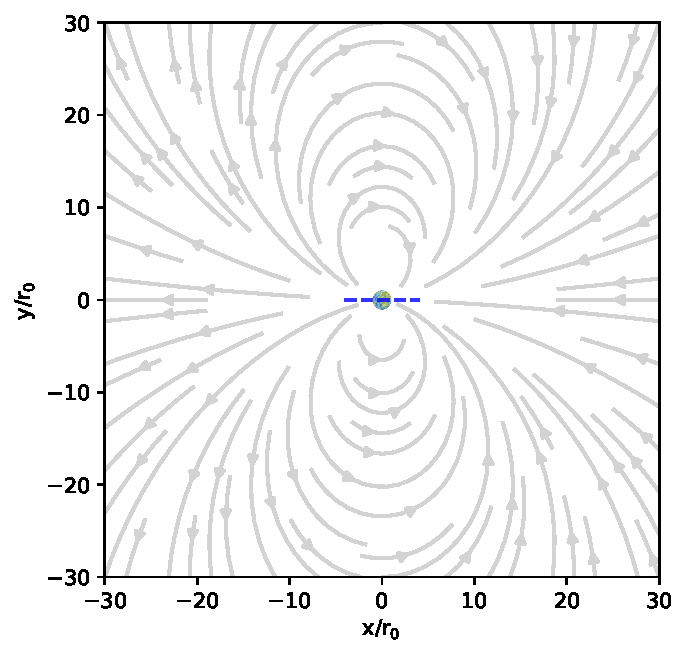
\includegraphics[width=0.49\textwidth]{../figures/report/magFieldXY}
    \caption{\textbf{Magnetic field produced by earth}\\The blue striped line represents the direction of \\earths magnetic moment (the length is scaled).}
    \label{fig:mag_field}
\end{figure}

\noindent Three different $\tilde{v_0}$ has been chosen according to \cite{solar_wind}, low, intermediate and high.
\begin{center}
\begin{tabular}{|c|c|c|c|c|c|c|}
\hline
    type & $\tilde{v_0}$ \\ 
\hline
    low & 250 km/s\\
    intermediate & 500 km/s\\
    high & 750 km/s\\
\hline
\end{tabular}
\label{table:constants}
\end{center}
\noindent For all starting points, $\tilde{\vectorbold{v_0}} \parallel \hat{\vectorbold{x}}$, and is sent towards earth. Since the magnetic field acts perpendicular to the trajectory, the protons should spiral around the field lines. This is observed in figure \ref{fig:low_trajectories}. It seems like the trajectories that start farther away oscillates more. 
\newpage
\begin{figure}[!htp]
    \centering
    \captionsetup{justification=centering}
    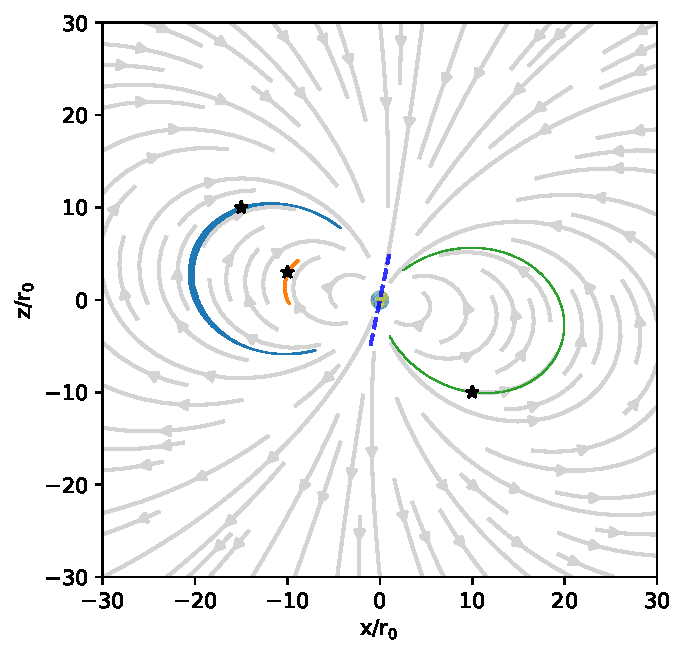
\includegraphics[width=0.49\textwidth]{../figures/report/trajectoriesLowXZ}
    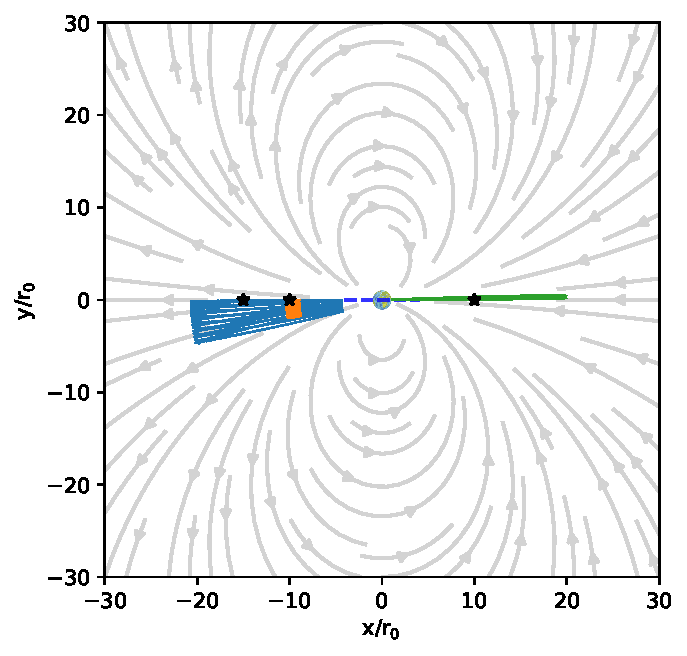
\includegraphics[width=0.49\textwidth]{../figures/report/trajectoriesLowXY}
    \caption{\textbf{Low velocity trajectories}\\Trajectories are represented by colored curves.\\Initial starting points are represented by black markers.}
    \label{fig:low_trajectories}
\end{figure}

\noindent Figure \ref{fig:intermediate_trajectories} illustrates intermediate velocity trajectories, with same starting points as in figure \ref{fig:low_trajectories}. The higher initial velocity makes the protons oscillate alot more. The blue and orange trajectory seems to have a periodic motion where it oscillates around the earth. Probably the green trajectory should also have a circular motion as the blue one, if one had solved the ODE for a longer time interval.
\begin{figure}[!htp]
    \centering
    \captionsetup{justification=centering}
    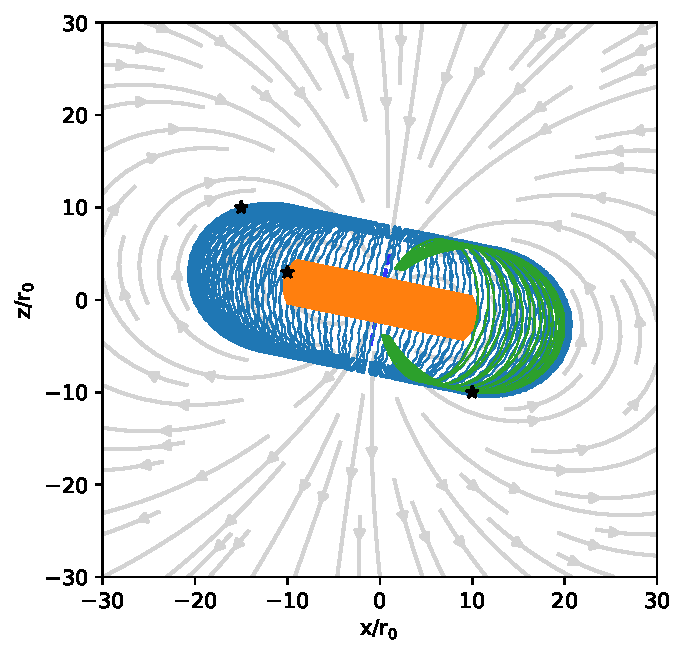
\includegraphics[width=0.49\textwidth]{../figures/report/trajectoriesIntermediateXZ}
    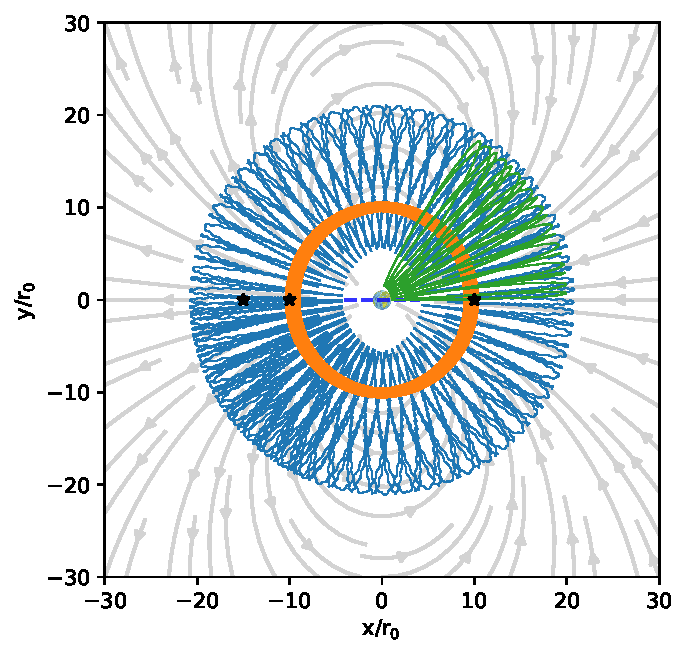
\includegraphics[width=0.49\textwidth]{../figures/report/trajectoriesIntermediateXY}
    \caption{\textbf{Intermediate velocity trajectories}}
    \label{fig:intermediate_trajectories}
\end{figure}

\newpage
\noindent The high velocity trajectories seem to be almost the same as for the intermediate velocitiy. One difference is that high velocity seems to produce more "squiggly" trajectories.
\begin{figure}[!htp]
    \centering
    \captionsetup{justification=centering}
    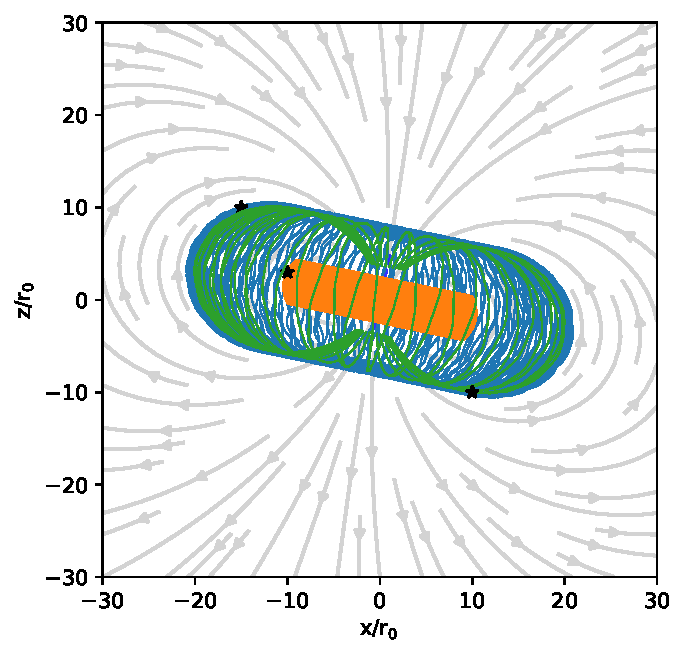
\includegraphics[width=0.49\textwidth]{../figures/report/trajectoriesHighXZ}
    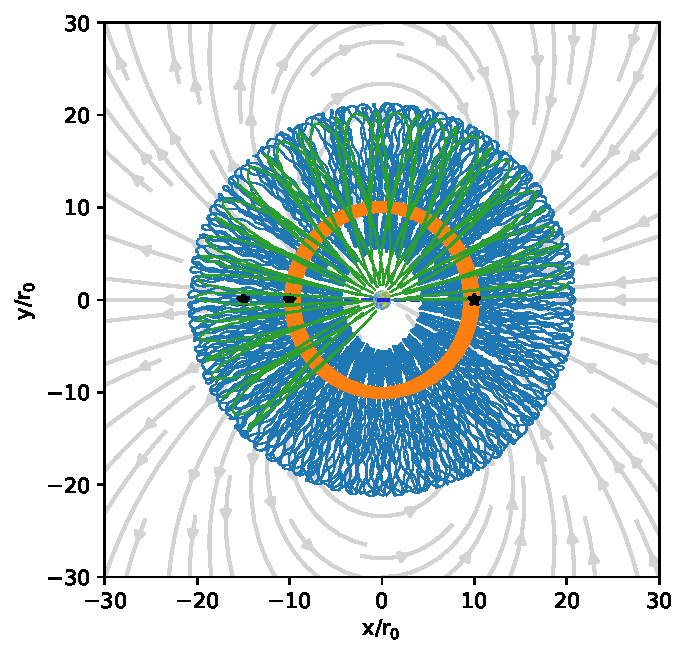
\includegraphics[width=0.49\textwidth]{../figures/report/trajectoriesHighXY}
    \caption{\textbf{High velocity trajectories}}
    \label{fig:high_trajectories}
\end{figure}

\noindent To verify that the solution converges, one can use the fact that magnetic fields do no work on classical charges. The energy should therefore remain constant. Normalized energy difference has been plotted in \ref{fig:energy}. The Runge-Kutta-Fehlberg method seems to hold the energy almost at zero, but probably a symplectic integrator would be a better choice.

\begin{figure}[!htp]
    \centering
    \captionsetup{justification=centering}
    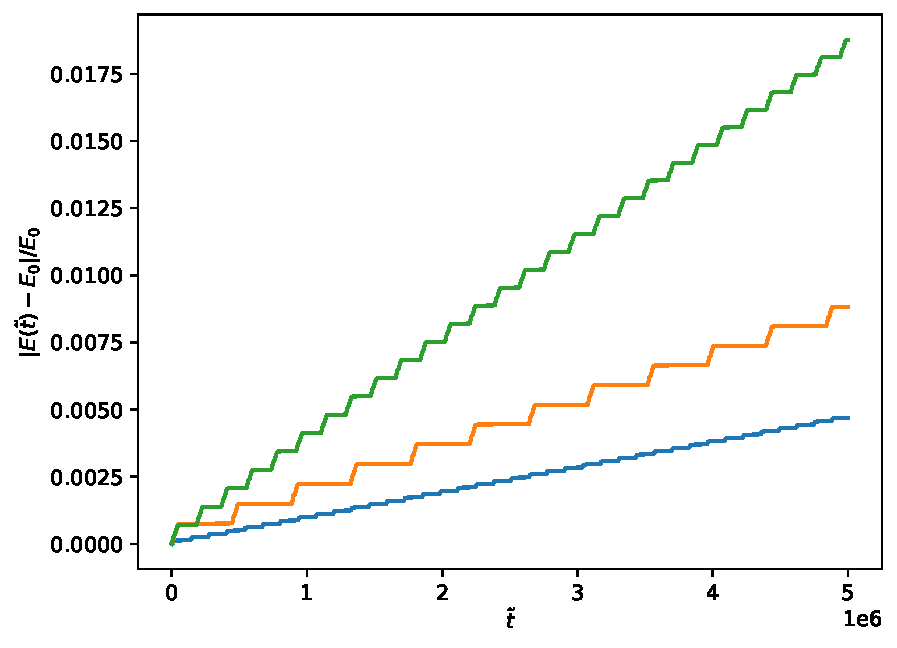
\includegraphics[width=0.45\textwidth]{../figures/report/energyDifference.pdf}
    \caption{\textbf{Normalized energy difference}}
    \label{fig:energy}
\end{figure}

\begin{thebibliography}{99}
    \bibitem{solar_wind} Solar wind, Wikipedia \\ \url{https://en.wikipedia.org/wiki/Solar_wind}
    \bibitem{erlensy_github} Syljuåsen, solar\_winds, \\\url{https://github.com/erlensy/solar_wind}
\end{thebibliography}
\end{document}
